\documentclass{ctexbeamer}
\usepackage{graphicx}
\usepackage{xcolor}
\usepackage{amssymb}
\usepackage{amsfonts}
\usepackage{pifont}
\usepackage{bm}
\usepackage{subcaption}
\def\E{\mathbb{E}}
\def\R{\mathbb{R}}
\DeclareMathOperator{\Vol}{Vol}
\newif\ifbeamer
\beamertrue

%further improvement
%background intro added Chen Chuan's work
%simulation add hierarchical method
%find suitable dataset to apply info-clustering
%Yang Li's suggestion: compared with other clustering method, the threshold is the same or not
%early stopping technique, complexity from n -> log(n)
\title{The Grand Canonical Ensemble}
%\author{Feng Zhao}
\date{\today}
\begin{document}
\begin{frame}
	\titlepage
\end{frame}
\begin{frame}{Outline}
    \tableofcontents
\end{frame}
\section{4.1 Equilibrium between 
a system and a particle-energy reservoir
}

\begin{frame}
\frametitle{巨正则系综}
\begin{itemize}
    \item 自变量:$\mu,V,T$
    \item 分布函数:$P_{r,s} \propto \exp(-\alpha N_r - \beta E_s)$
    \item 参数:$\alpha=-\frac{\mu}{kT}, \beta = \frac{1}{kT}$
\end{itemize}

\end{frame}
\section{4.2 A system in the grand canonical ensemble
}
\begin{frame}
    \frametitle{巨正则系综概率分布的推导}
    \begin{enumerate}
        \item 最可几方法:拉格朗日乘子法求带约束的优化问题的最大值
        \item 平均值方法
    \end{enumerate}
    
    \end{frame}
\section{4.3 Physical significance of the various
statistical quantities}
\begin{frame}{巨正则系综的热力学公式}
    \begin{enumerate}
        \item 巨配分函数:
        $\mathcal{Q}(z,V,T)
         \sum_{N_r=0}^{\infty}
         z^{N_r} Q_{N_r}(V,T)$,其中
         $z=\exp(\frac{\mu}{kT})$。
         \item 压强公式: $P=\frac{kT}{V} \ln \mathcal{Q}$
         \item 内能公式: $U=-\frac{\partial \ln \mathcal{Q}}{\partial \beta}$
         \item 粒子数公式:
         $N=z\frac{\partial \ln \mathcal{Q}}{\partial z}$
        \end{enumerate}
\end{frame}
\section{4.4 Examples}
\begin{frame}{由巨正则系综推导4个分子系统的热力学公式}
    \begin{enumerate}
        \item 动能 $\mathcal{Q} = \exp(zVf(T))$
        \begin{enumerate}
            \item 单原子理想气体 $f(T) = (2\pi m kT)^{3/2}/h^3$
            \item 极度相对性气体 (extreme relativistic gas)
            $f(T) \propto T^3 $
        \end{enumerate}
        \item 势能 $\mathcal{Q} = [1-z\phi(T)]^{-1}$
        \begin{enumerate}
            \item 量子力学的谐振子 $\phi(T)=[2\sinh(\frac{\hbar w}{2kT})]^{-1}$
            \item 经典谐振子 $ \phi(T) = \frac{kT}{\hbar w}$
        \end{enumerate}
    \end{enumerate}
\end{frame}
\section{4.5 Density and energy fluctuations in the grand canonical ensemble}
\begin{frame}{巨正则系综的能量和密度涨落}
    \begin{itemize}
        \item 密度:$n=N/V$
        \item 在平均值附近的能量、密度涨落很小
        \item 巨正则系综与正则系综导出相同的热力学公式
    \end{itemize}
\end{frame}
\section{4.6 Thermodynamic phase diagrams}
\begin{frame}{热力学相图}  
    \begin{columns}
		\column{5cm}
		\begin{figure}
			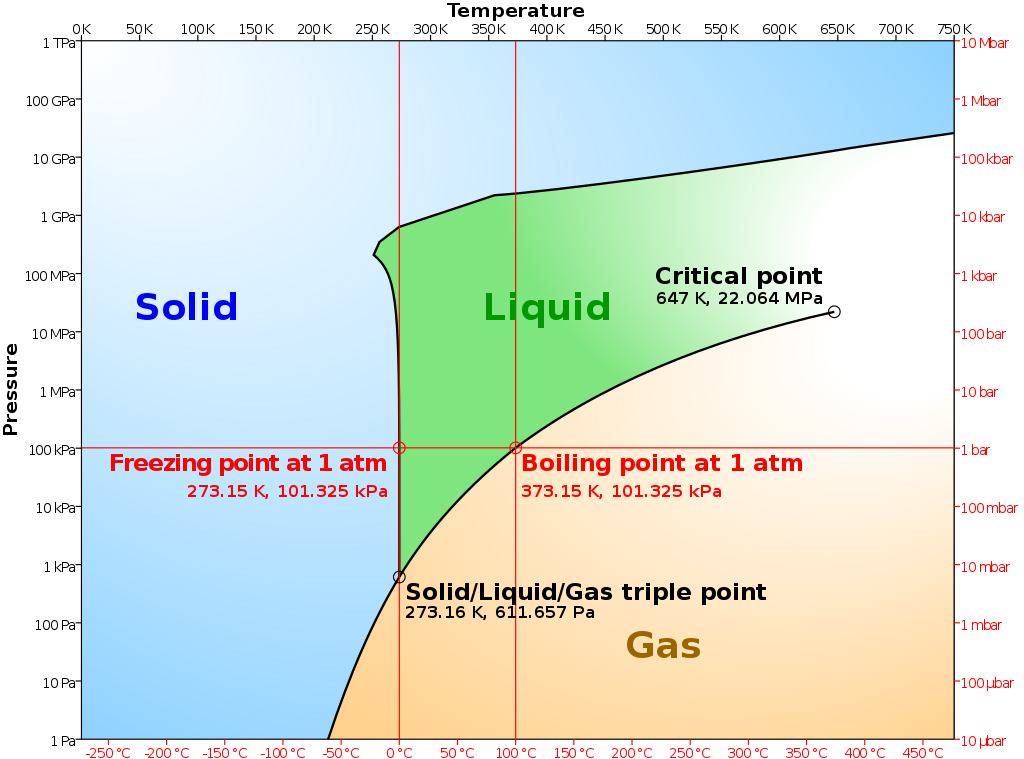
\includegraphics[width=5cm]{phase_trans.png}
			\caption{水的相图}
		\end{figure}
		\column{5cm}
\begin{itemize}
    \item     两相平衡条件:化学势相等
    \item 一阶相变公式(以液汽共存为例)
\begin{equation}
    \frac{dP}{dT} = \frac{LP}{k T^2}
\end{equation}
\end{itemize}	
	\end{columns}
\end{frame}
\end{document}
